\documentclass{article}
	\usepackage[UTF8]{ctex}
	\usepackage{amsmath}
	\usepackage{graphicx}
	\usepackage{underscore}
	\usepackage{geometry}
	\usepackage{anysize}
	\usepackage{verbatim}
	\usepackage{caption}
	\date{}
	\title{三方坐镇 \\ [2ex] \begin{large} 
	时间限制：C/C++ 1秒，其他语言2秒 \\
	空间限制：C/C++ 32.000MB，其他语言64.000MB 	\\
	Special Judge,64bit IO Format: \%lld
 			\end{large} }
	\geometry{top=10mm,bottom=15mm,left=25mm,right=25mm}
	\setlength{\abovedisplayskip}{3pt}
	
	\begin{document}
		\maketitle \vspace{-50pt}
		
		\section*{题目描述}
		\indent 在二维平面上，有三个圆，请求出三个圆的覆盖面积(重叠部分只计算一次)。特别的，若三个圆两两相交，则输出-1。\\
		\indent 两圆相交：设圆1和圆2的覆盖范围分别为$S_{1}$和$S_{2}$ ，有$S_{1}\cup S_{2} \neq S_{1}$ ,  $S_{1}\cup S_{2} \neq S_{2}$ 和 $S_{1}\cap S_{2} \neq \emptyset $。

		\section*{输入描述}
			\noindent 第1行输入数据组数$n$($1 \le n \le 100$)。
			接下来对于每组数据，输入3行，每行$3$个数字$x,y,r$($-100 \le x,y \le 100$,$0 < r \le 100$,x,y,r的小数位数小于等于3)，分别为圆心的横坐标、纵坐标和圆的半径大小。 

		\section*{输出描述}
			\noindent 对于每组数据，若三个圆两两相交，则输出-1，否则输出三个圆的覆盖面积。本题采用Special Judge，要求输出结果(-1除外)与正确结果相差小于$10^{-2}$。其中$\pi=3.14159265358979\dots$。
			
		\section*{示例1}
			\subsection*{输入}
\noindent
4	\\
0 0 3	\\
0 0 5	\\
0 0 7	\\
-2 -2 1	\\
1 1 2	\\
6 6 3	\\
-5 0 4	\\
-5 4 4	\\	
2.5 2.5 2.5	\\
0 0 3	\\
4 0 3	\\
2 3.5 3

			\subsection*{输出}
\noindent
153.94	\\
43.98		\\
100.51	\\
-1

			\subsection*{说明}
			\noindent 前三个结果输出不唯一，最后一个结果输出唯一。图片位于第三页。\\

\begin{figure}[h]

\begin{minipage}[t]{0.5\linewidth}
\centering

\includegraphics[width=3in]{1.png}
\caption*{圆1}
\end{minipage}%
\begin{minipage}[t]{0.5\linewidth}
\centering

\includegraphics[width=3in]{2.png}
\caption*{面积1}
\end{minipage}

\begin{minipage}[t]{0.5\linewidth}
\centering

\includegraphics[width=3in]{3.png}
\caption*{圆2}
\end{minipage}%
\begin{minipage}[t]{0.5\linewidth}
\centering

\includegraphics[width=3in]{4.png}
\caption*{面积2}
\end{minipage}

\begin{minipage}[t]{0.5\linewidth}
\centering
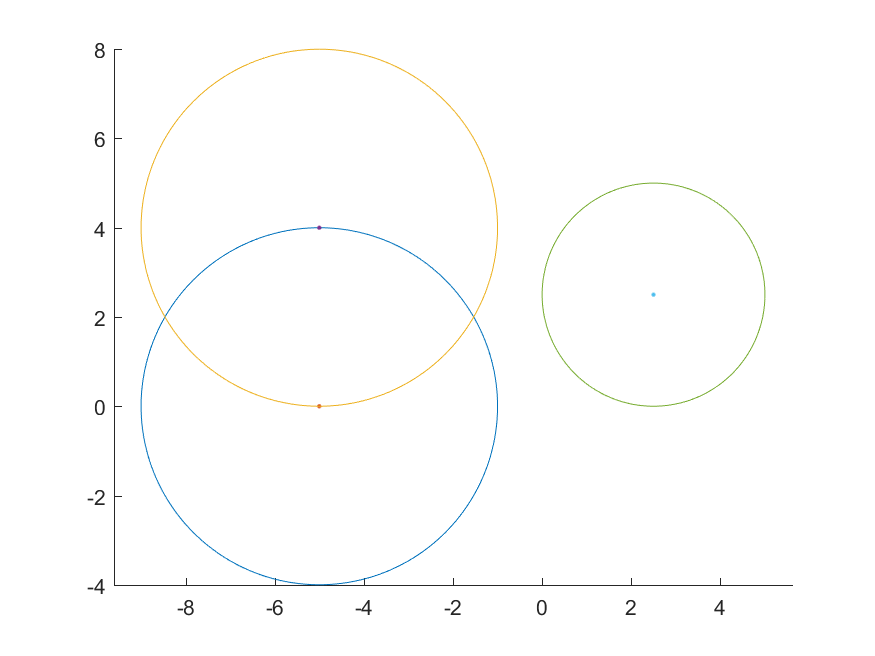
\includegraphics[width=3in]{5.png}
\caption*{圆3}
\end{minipage}%
\begin{minipage}[t]{0.5\linewidth}
\centering
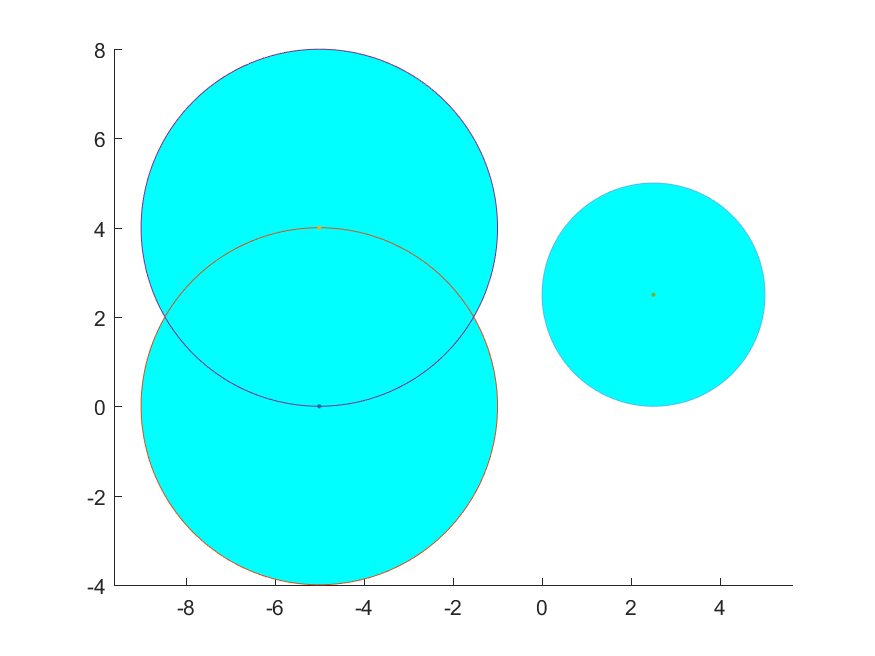
\includegraphics[width=3in]{6.png}
\caption*{面积3}
\end{minipage}

\begin{minipage}[t]{0.5\linewidth}
\centering
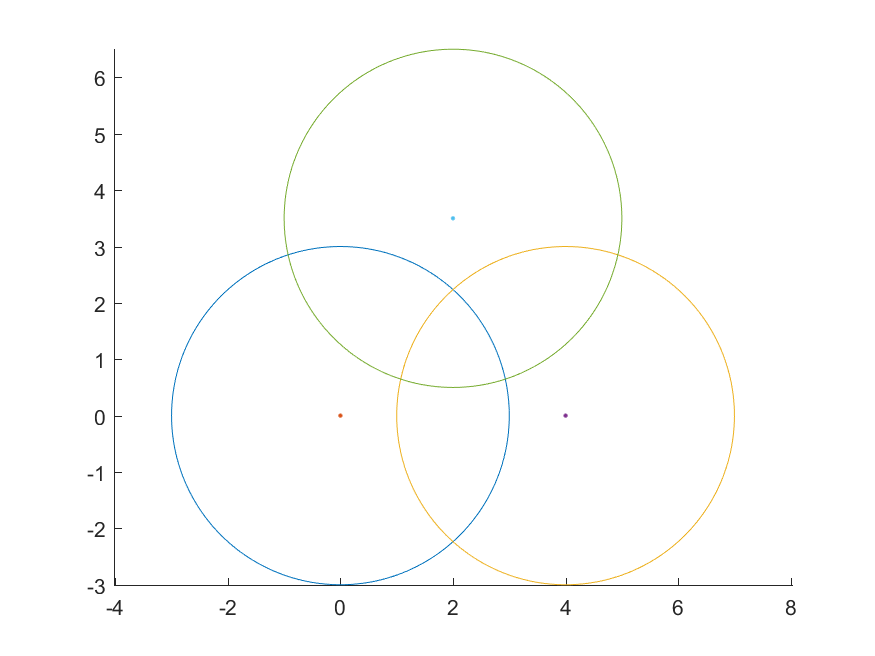
\includegraphics[width=3in]{7.png}
\caption*{圆4}
\end{minipage}%
\begin{minipage}[t]{0.5\linewidth}
\centering
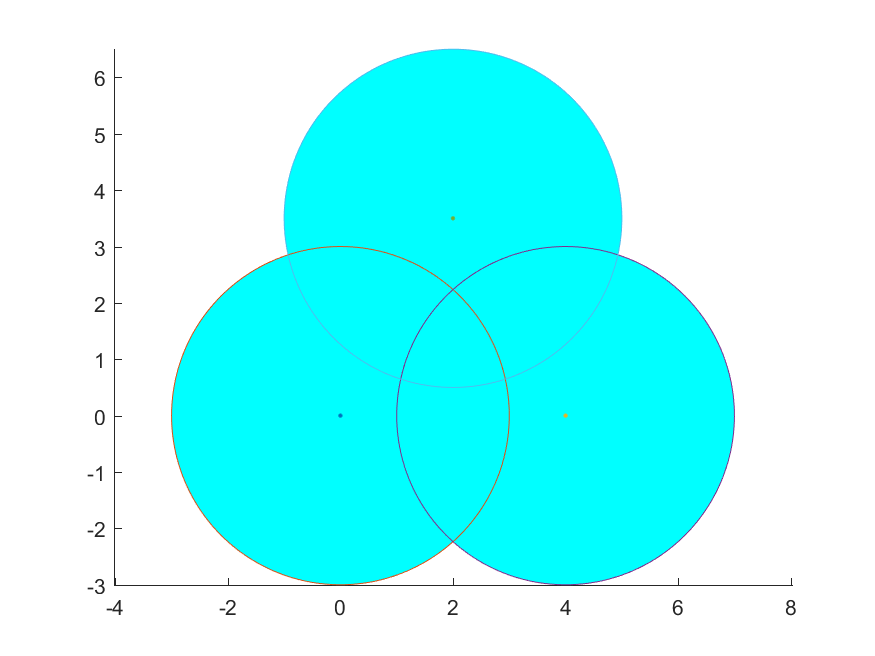
\includegraphics[width=3in]{8.png}
\caption*{面积4}
\end{minipage}
\end{figure}

	\section*{也许需要用到的函数}
		\subsection*{c/c++}
			在math.h/cmath库中，\\
			\indent double sin( double arg );\\
			\indent 功能： 函数返回参数arg的正弦值，arg以弧度表示给出。\\\\
			\indent double asin( double arg );\\
			\indent 功能：函数返回参数arg的反正弦值，参数arg 应当在-1和1之间。\\\\
			\indent double pow( double base, double exp );\\
			\indent 功能：函数返回以参数base为底的exp次幂。如果base为零或负和exp小于等于零或非整数时，产生域错误。如果溢出，产生范围错误。 

		\subsection*{java}
			在java.lang.Math类中，存在sin,asin,pow函数，使用方法与c/c++类似。

		\subsection*{python}
			在math类中，存在sin,asin,pow函数，使用方法与c/c++类似。
			
	\section*{备注}
		\indent 对几何学有兴趣的同学不妨研究一下三个圆互相相交的情况。\\

	\end
	{document}	
